\documentclass{beamer}
\usepackage[utf8]{inputenc}

\usetheme{Madrid}
\usecolortheme{default}
\usepackage{amsmath,amssymb,amsfonts,amsthm}
\usepackage{txfonts}
\usepackage{tkz-euclide}
\usepackage{listings}
\usepackage{adjustbox}
\usepackage{array}
\usepackage{tabularx}
\usepackage{gvv}
\usepackage{lmodern}
\usepackage{circuitikz}
\usepackage{tikz}
\usepackage{graphicx}

\setbeamertemplate{page number in head/foot}[totalframenumber]

\usepackage{tcolorbox}
\tcbuselibrary{minted,breakable,xparse,skins}



\definecolor{bg}{gray}{0.95}
\DeclareTCBListing{mintedbox}{O{}m!O{}}{%
  breakable=true,
  listing engine=minted,
  listing only,
  minted language=#2,
  minted style=default,
  minted options={%
    linenos,
    gobble=0,
    breaklines=true,
    breakafter=,,
    fontsize=\small,
    numbersep=8pt,
    #1},
  boxsep=0pt,
  left skip=0pt,
  right skip=0pt,
  left=25pt,
  right=0pt,
  top=3pt,
  bottom=3pt,
  arc=5pt,
  leftrule=0pt,
  rightrule=0pt,
  bottomrule=2pt,
  toprule=2pt,
  colback=bg,
  colframe=orange!70,
  enhanced,
  overlay={%
    \begin{tcbclipinterior}
    \fill[orange!20!white] (frame.south west) rectangle ([xshift=20pt]frame.north west);
    \end{tcbclipinterior}},
  #3,
}
\lstset{
    language=C,
    basicstyle=\ttfamily\small,
    keywordstyle=\color{blue},
    stringstyle=\color{orange},
    commentstyle=\color{green!60!black},
    numbers=left,
    numberstyle=\tiny\color{gray},
    breaklines=true,
    showstringspaces=false,
}
%------------------------------------------------------------
%This block of code defines the information to appear in the
%Title page
\title %optional
{1.5.20}
\date{August 29,2025}


\author 
{Jnanesh Sathisha karmar - EE25BTECH11029}



\begin{document}



\frame{\titlepage}
\begin{frame}{Question}
The midpoint of the line segment joining $\vec{A}\brak{2a, 4}$ and $\vec{B}\brak{-2, 3b}$ is \brak{1, 2a + 1}. Find
the values of a and b.
\end{frame}



\begin{frame}{Equation}

The midpoint M of line segment AB, with $\vec{A}\brak{x_1, y_1}$ and $\vec{B}\brak{x_2, y_2}$, is:
\begin{align}
	\vec{M}=\frac{\vec{A}+\vec{B}}{2}=\frac{\myvec{x_1\\y_1} + \myvec{x_2\\y_2}}{2}
\end{align}

\end{frame}

\begin{frame}{Theoretical Solution}

Given details:
\begin{align}
    \vec{A}=\myvec{2a\\4}  \vec{B}=\myvec{-2\\3b} \vec{M}=\myvec{1\\2a+1}
\end{align}
\end{frame}

\begin{frame}{Theoretical Solution}

Substituting the points:
\begin{align}
\frac{\myvec{2a\\4} + \myvec{-2\\3b}}{2}=\myvec{\frac{2a-2}{2}\\ \frac{\brak{4+3b}}{2}}
\end{align}

\end{frame}


\begin{frame}{Theoretical Solution}
Equating coordinates, we get two equations:
\begin{align}
\frac{2a - 2}{2} &= 1 \\
\frac{4 + 3b}{2} &= 2a + 1
\end{align}

\end{frame}
\begin{frame}{Theoretical Solution}
Using \brak{3} 
\begin{align}
    a=2
\end{align}
Using \brak{3} and \brak{6}
\begin{align}
    b=2
\end{align}
Therefore Values of $a$ and $b$ are both $2$
\end{frame}

\begin{frame}[fragile]
    \frametitle{C Code (1) - Function to generate a line segment }

    \begin{lstlisting}

#include <stdio.h>

void line_segment_gen(double *X, double *Y, double *A, double *B, int n)
{
    double dx = (B[0] - A[0]) / (double)n;
    double dy = (B[1] - A[1]) / (double)n;

    for (int i = 0; i <= n; i++)
    {
        X[i] = A[0] + dx * i;
        Y[i] = A[1] + dy * i;
    }
}
    \end{lstlisting}
\end{frame}


\begin{frame}[fragile]
    \frametitle{Python Code - Using Shared Object}
    \begin{lstlisting}

import ctypes
import numpy as np
import matplotlib.pyplot as plt

# Load shared library
lib = ctypes.CDLL("./line_segment.so")

# Define argument types for the C function
lib.line_segment_gen.argtypes = [
    np.ctypeslib.ndpointer(dtype=np.double, ndim=1, flags="C_CONTIGUOUS"),  # X
    np.ctypeslib.ndpointer(dtype=np.double, ndim=1, flags="C_CONTIGUOUS"),  # Y
    np.ctypeslib.ndpointer(dtype=np.double, ndim=1, flags="C_CONTIGUOUS"),  # A
   



\end{lstlisting}
\end{frame}

\begin{frame}[fragile]
    \frametitle{Python Code - Using Shared Object}
    \begin{lstlisting}
 np.ctypeslib.ndpointer(dtype=np.double, ndim=1, flags="C_CONTIGUOUS"),  # B
    ctypes.c_int
]
# Define start & end points
A = np.array([4.0, 4.0], dtype=np.double)    # Point (4,4)
B = np.array([-2.0, 6.0], dtype=np.double)   # Point (-2,6)
n = 20  # number of segments

# Allocate space for results
X = np.zeros(n+1, dtype=np.double)
Y = np.zeros(n+1, dtype=np.double)

# Call the C function
lib.line_segment_gen(X, Y, A, B, n)

# Compute midpoint
midpoint = np.array([(A[0] + B[0]) / 2, (A[1] + B[1]) / 2])

\end{lstlisting}
\end{frame}
\begin{frame}[fragile]
    \frametitle{Python Code - Using Shared Object}
    \begin{lstlisting}
# --------- Plotting ---------
plt.figure(figsize=(6,6))

# Draw line segment
plt.plot(X, Y, 'b-', label="Line segment")

# Mark endpoints
plt.scatter(A[0], A[1], color='red', s=80, zorder=3, label="Point A (4,4)")
plt.scatter(B[0], B[1], color='green', s=80, zorder=3, label="Point B (-2,6)")

# Mark midpoint
plt.scatter(midpoint[0], midpoint[1], color='purple', s=100, marker='x', zorder=4, label="Midpoint (1,5)")





\end{lstlisting}
\end{frame}
\begin{frame}[fragile]
    \frametitle{Python Code - Using Shared Object}
    \begin{lstlisting}
# Labels & grid
plt.xlabel("X")
plt.ylabel("Y")
plt.title("Line segment between A(4,4) and B(-2,6) with Midpoint")
plt.legend()
plt.grid(True)
plt.axis("equal")
plt.savefig('figs/line_segment.png')
subprocess.run(shlex.split("termux-open figs/line_segment.png"))
\end{lstlisting}
\end{frame}


\begin{frame}{Plot-Using Both C and Python}
    \centering
    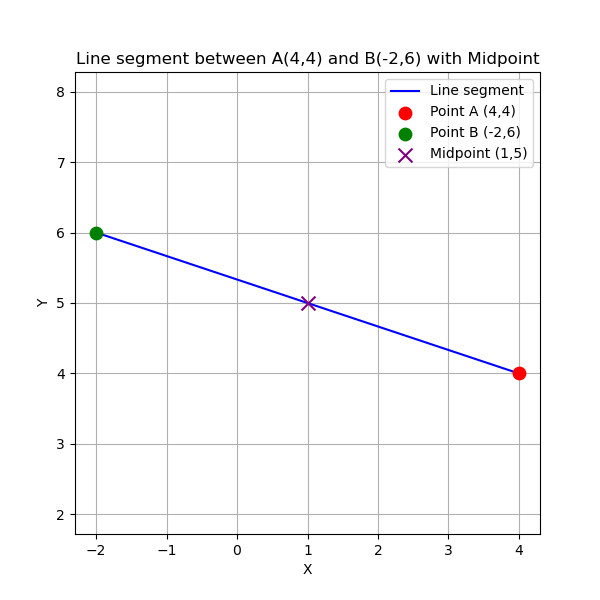
\includegraphics[width=\columnwidth, height=0.8\textheight, keepaspectratio]{figs/line_segment.png}     
\end{frame}

\begin{frame}[fragile]
    \frametitle{Python Code}
    \begin{lstlisting}
import numpy as np
import matplotlib.pyplot as plt

# Define points
A = np.array([4.0, 4.0])
B = np.array([-2.0, 6.0])

# Generate line segment points
n = 20
X = np.linspace(A[0], B[0], n+1)
Y = np.linspace(A[1], B[1], n+1)


\end{lstlisting}
\end{frame}

\begin{frame}[fragile]
    \frametitle{Python Code }
    \begin{lstlisting}
# --------- Plotting ---------
plt.figure(figsize=(6,6))

# Line
plt.plot(X, Y, 'b-', label="Line segment")

# Endpoints
plt.scatter(A[0], A[1], color='red', s=80, zorder=3, label="Point A (4,4)")
plt.scatter(B[0], B[1], color='green', s=80, zorder=3, label="Point B (-2,6)")

# Midpoint
plt.scatter(midpoint[0], midpoint[1], color='purple', s=100, marker='x', zorder=4, label="Midpoint (1,5)")


\end{lstlisting}
\end{frame}

\begin{frame}[fragile]
    \frametitle{Python Code }
    \begin{lstlisting}
    # Midpoint
midpoint = (A + B) / 2


# Labels & grid
plt.xlabel("X")
plt.ylabel("Y")
plt.title("Line segment between A(4,4) and B(-2,6) with Midpoint")
plt.legend()
plt.grid(True)
plt.axis("equal")
plt.savefig('figs/line_segment2.png')
subprocess.run(shlex.split("termux-open figs/line_segment2.png"))

\end{lstlisting}
\end{frame}




\begin{frame}{Plot-Using only Python}
    \centering
    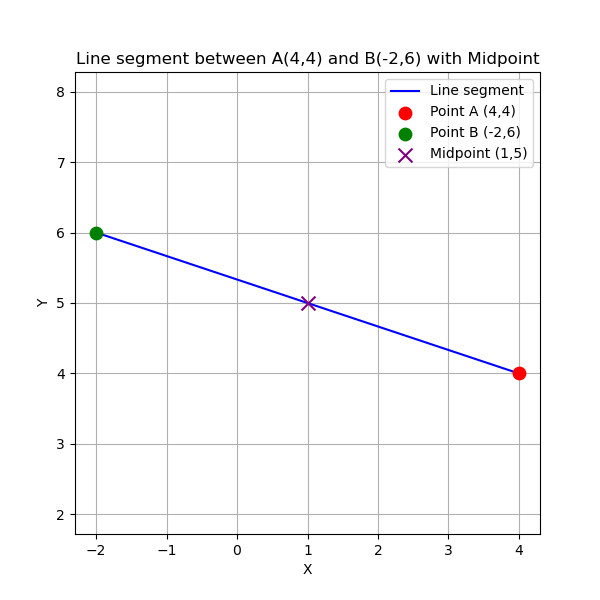
\includegraphics[width=\columnwidth, height=0.8\textheight, keepaspectratio]{figs/line_segment2.png}     
\end{frame}


\end{document}